\newpage
\section{Планирование траекторий движения}
Для выполнения парковочного маневра система строит траекторию, показанную на рисунке~\ref{img_planned_trajectory}.
Координаты зеленых точек на нем становятся известными после выполнения этапа картирования, остальных~--- рассчитываются после с учетом ширины робота~$H$, параметров~$\delta_1$ и $\delta_2$, задаваемых системе перед началом ее работы вручную, удвоенного минимального радиуса дуги, по которой может пройти робот, $R$ и некоторых математических соотношений.
Из последних стоит отметить лишь уравнения, совместное решение которых дает координаты $(x_5, y_5)$~--- координаты точки касания нижней из дуг и прямой, на которой лежит отрезок, ограниченный точками с координатами~$(x_3, y_3)$ и $(x_5, y_5)$:
\begin{equation}
    \left\{
    \begin{aligned}
        & (x_7 - x_5)^2 + (y_7 - y_5)^2 = R^2, \\
        & \frac{y_4 - y_5}{x_4 - x_5} \cdot \frac{y_5 - y_7}{x_5 - x_7} = -1 \ldotp
    \end{aligned}
    \right.
\end{equation}
Задача же определения координат остальных точек авторам представляется тривиальной.

\begin{figure}[h!]
    \centering
    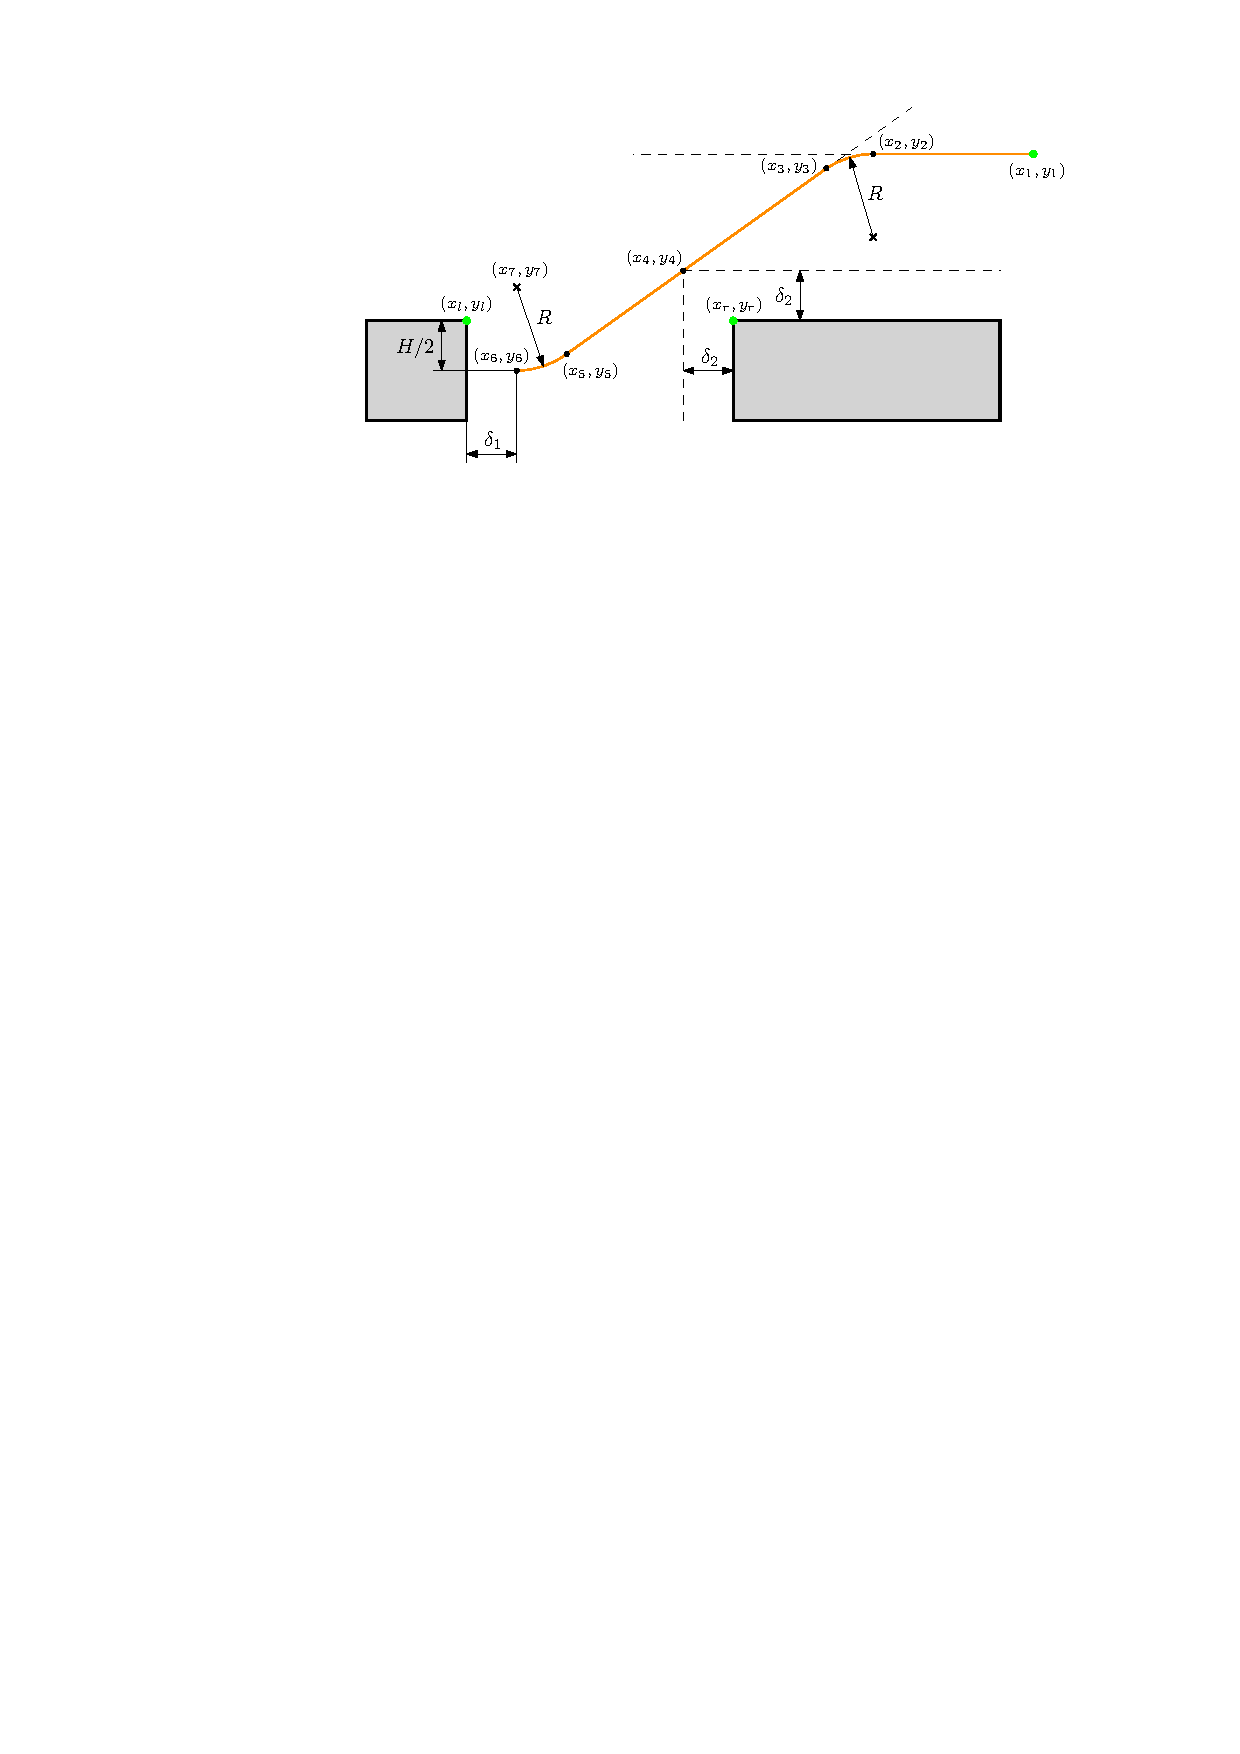
\includegraphics[width=\textwidth]{planned_trajectory.pdf}
    \vspace{0cm}
    \caption{Пояснения к принципам планирования траектории парковочного маневра.}
    \label{img_planned_trajectory}
\end{figure}

Пример траектории, спланированной благодаря созданному авторами ПО, можно видеть на рисунке~\ref{img_scilab_trajectory_maker}.

\begin{figure}[h!]
    \centering
    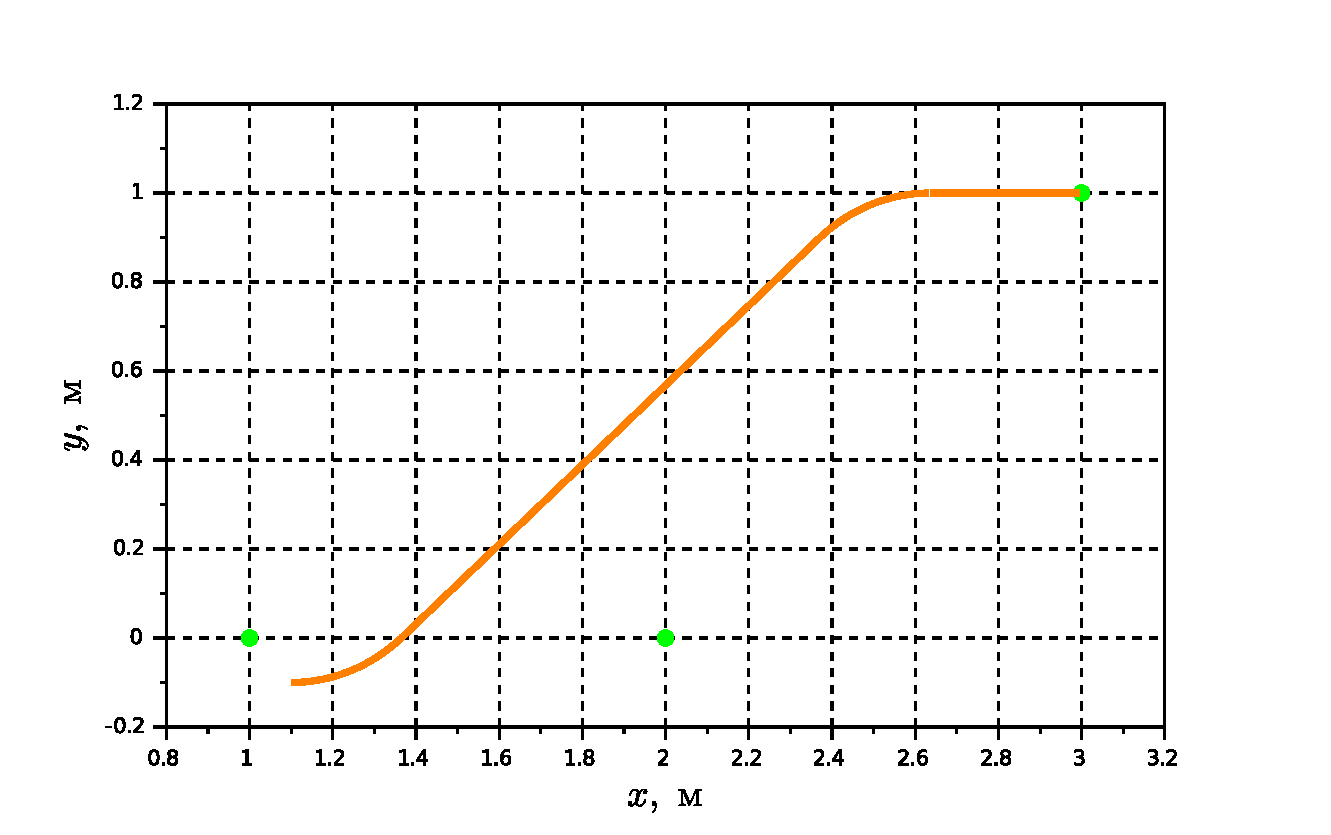
\includegraphics[width=0.8\textwidth]{scilab_trajectory_maker.pdf}
    \caption{Пример спланированной траектории движения.}
    \label{img_scilab_trajectory_maker}
\end{figure}

\newpage \mbox{} \newpage